\section*{Terminal}

%% Hacer el ejercicio de tomar la captura de pantalla 
%%  a la terminal y señalar las partes que salen 

\subsection*{Comandos Basicos}



%% Para cada uno de estos comandos incluyan una captura de 
%%  pantalla de su funcionamiento.
\begin{itemize}
    \item \textbf{ls} con al menos 3 banderas adicionales
    \begin{center}
        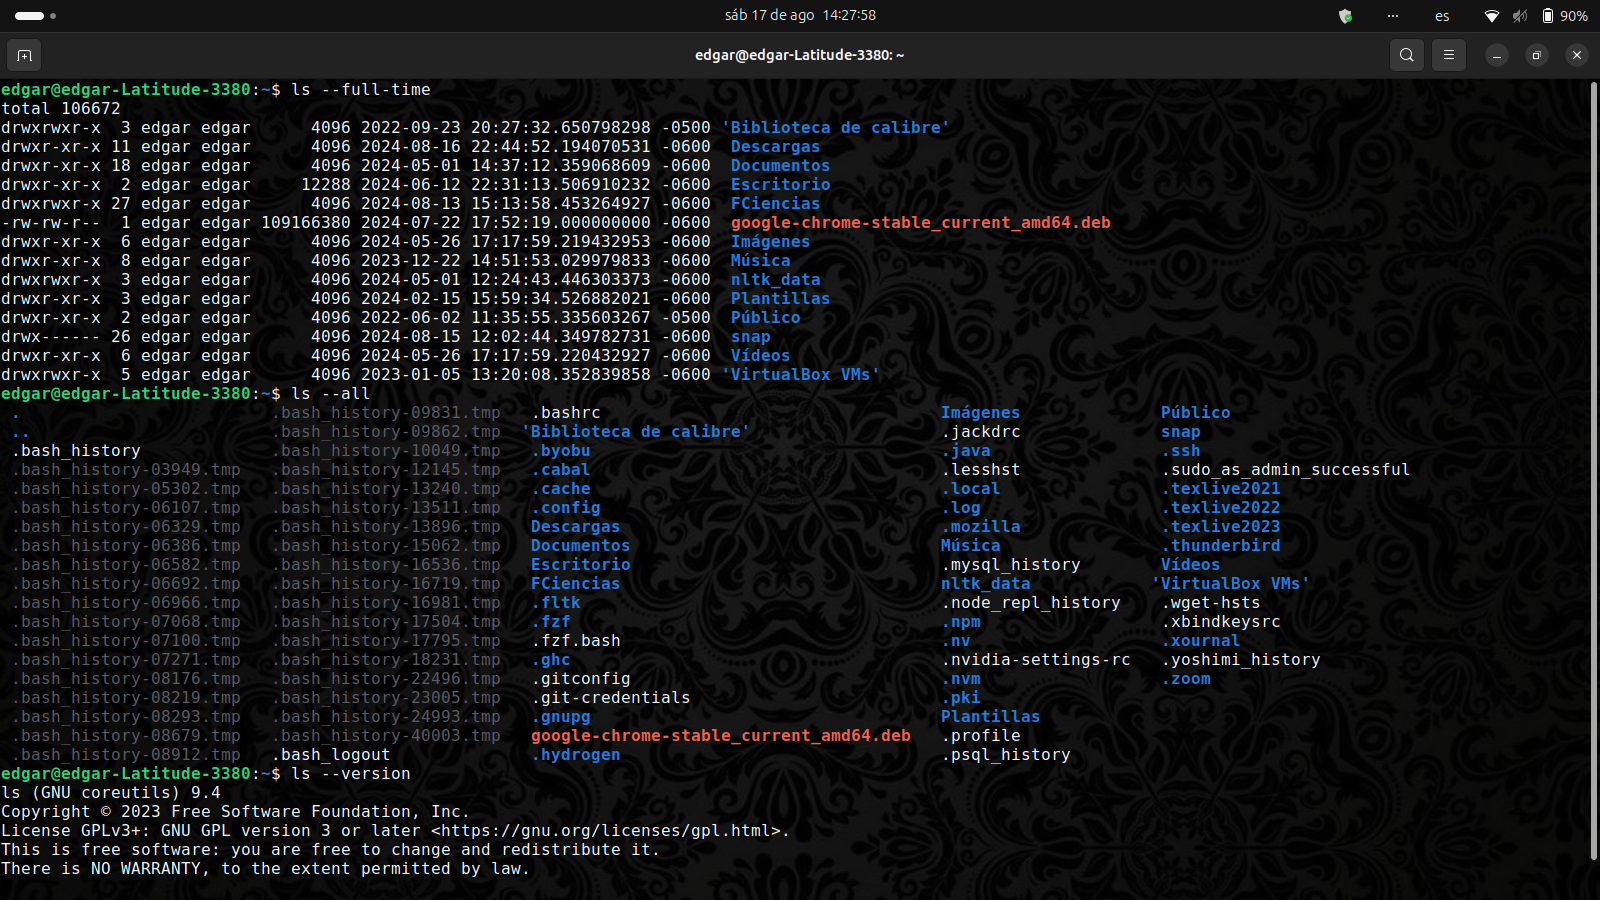
\includegraphics[width=10cm]{IMAGE/ls.png}
    \end{center}
    \begin{itemize}
        \item \texttt{ls --full-time}: Muestra detalles completos de archivos, incluyendo fecha y hora con segundos.
        \item \texttt{ls -al}: Lista todos los archivos, incluidos los ocultos, en un formato detallado.
        \item \texttt{ls --version}: Muestra la versión del comando \texttt{ls}.
    \end{itemize}

    
    \item \textbf{man} con al menos 3 banderas adicionales
    \begin{center}
        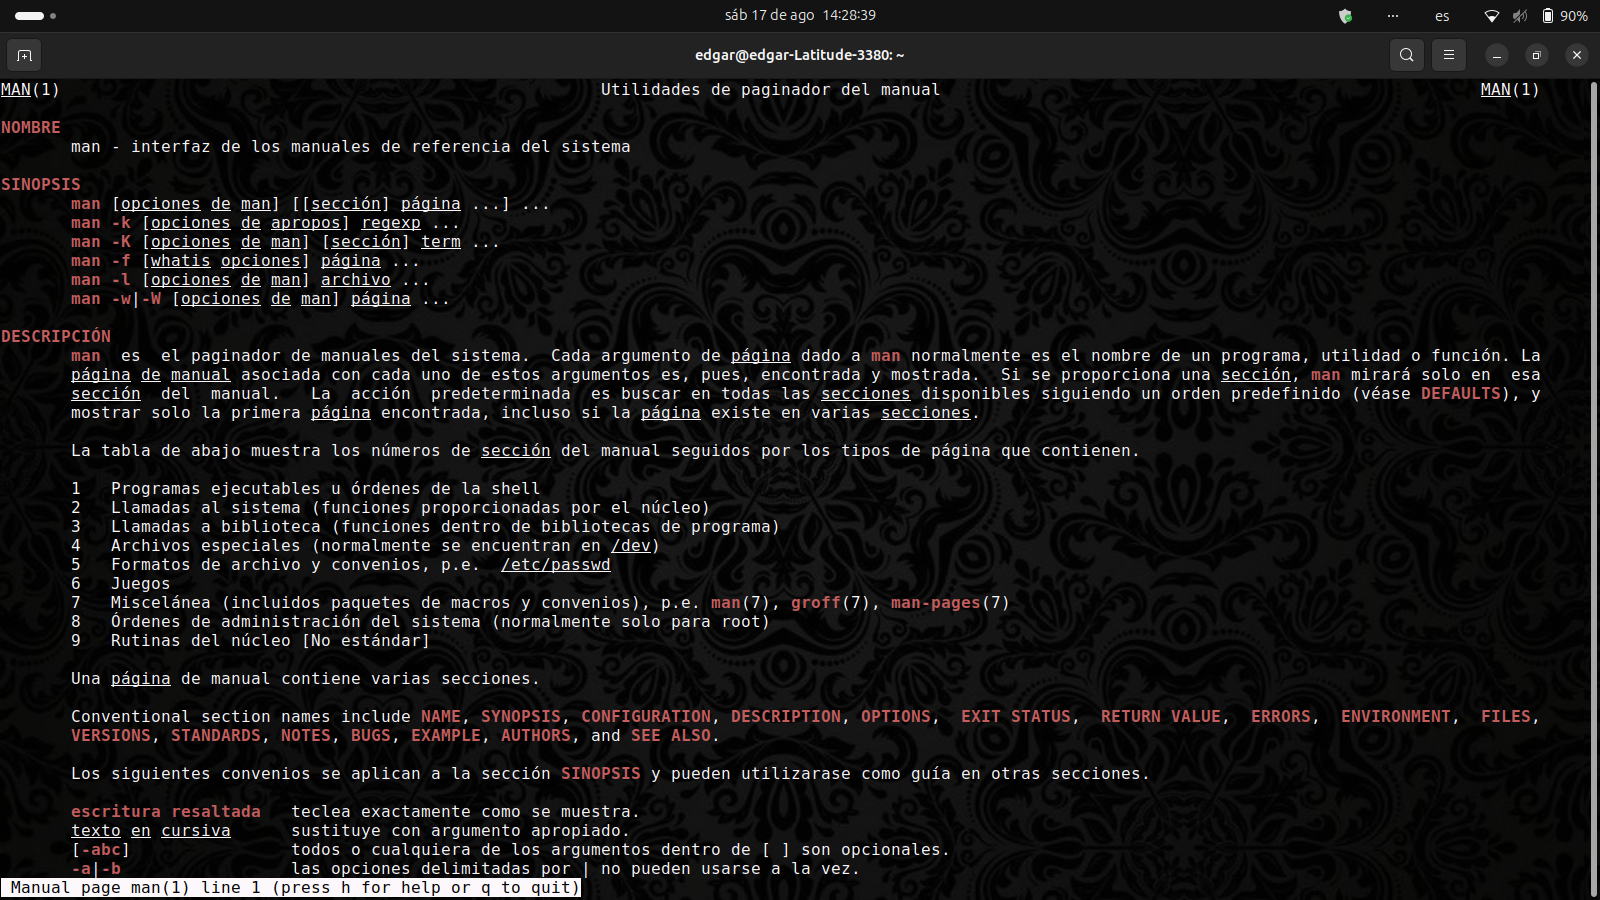
\includegraphics[width=10cm]{IMAGE/man-man.png}
    \end{center}
    \begin{center}
        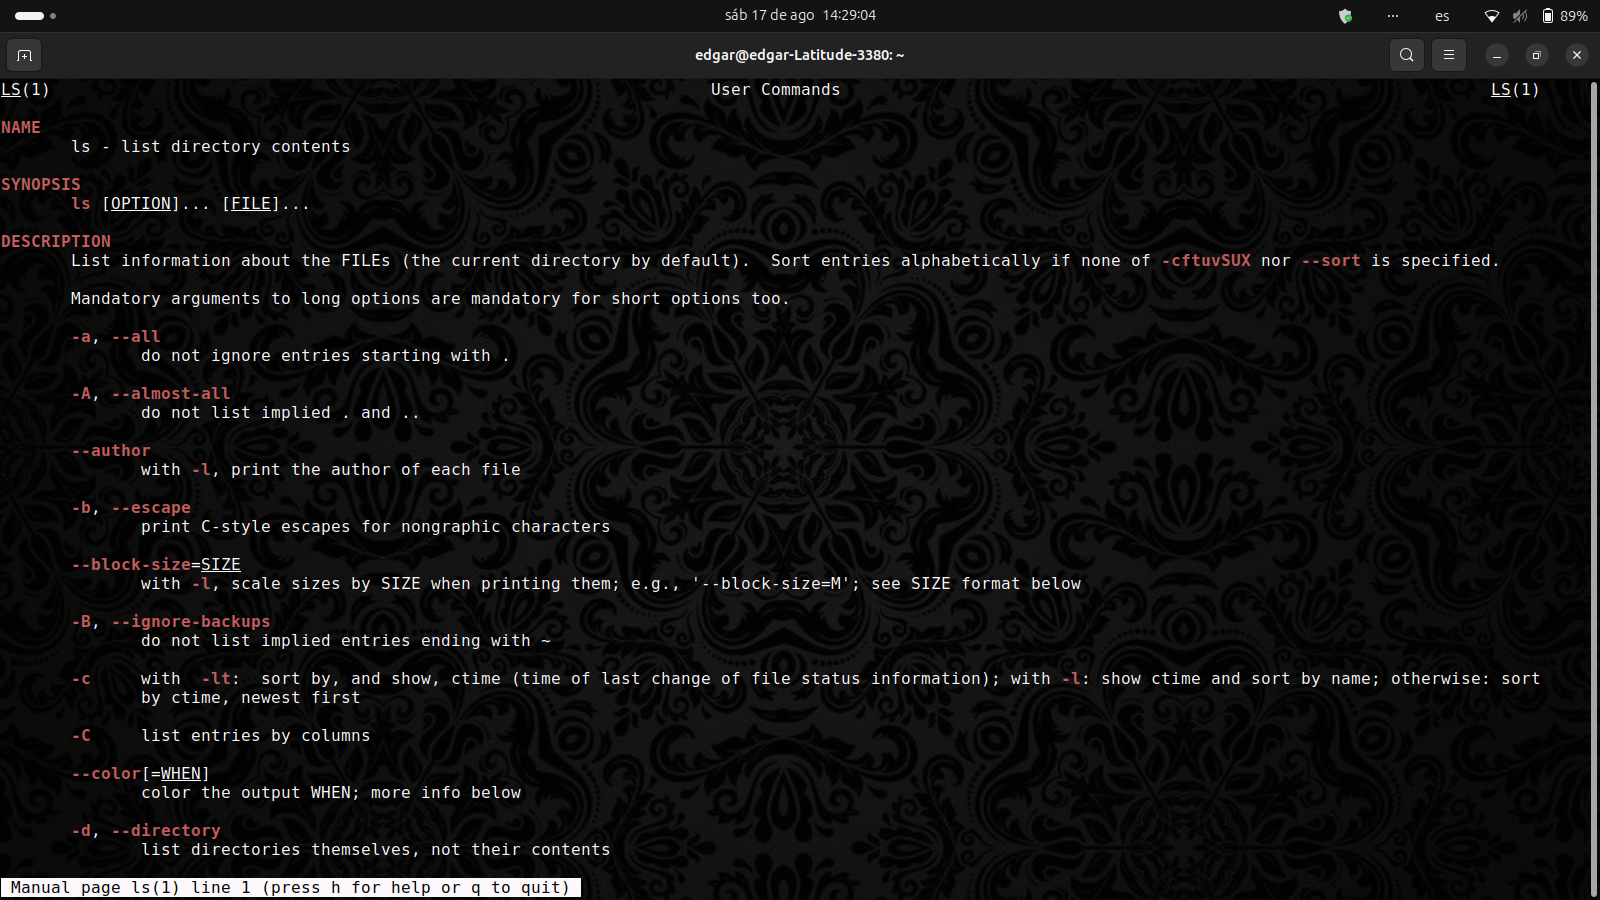
\includegraphics[width=10cm]{IMAGE/man-ls.png}
    \end{center}
    \begin{center}
        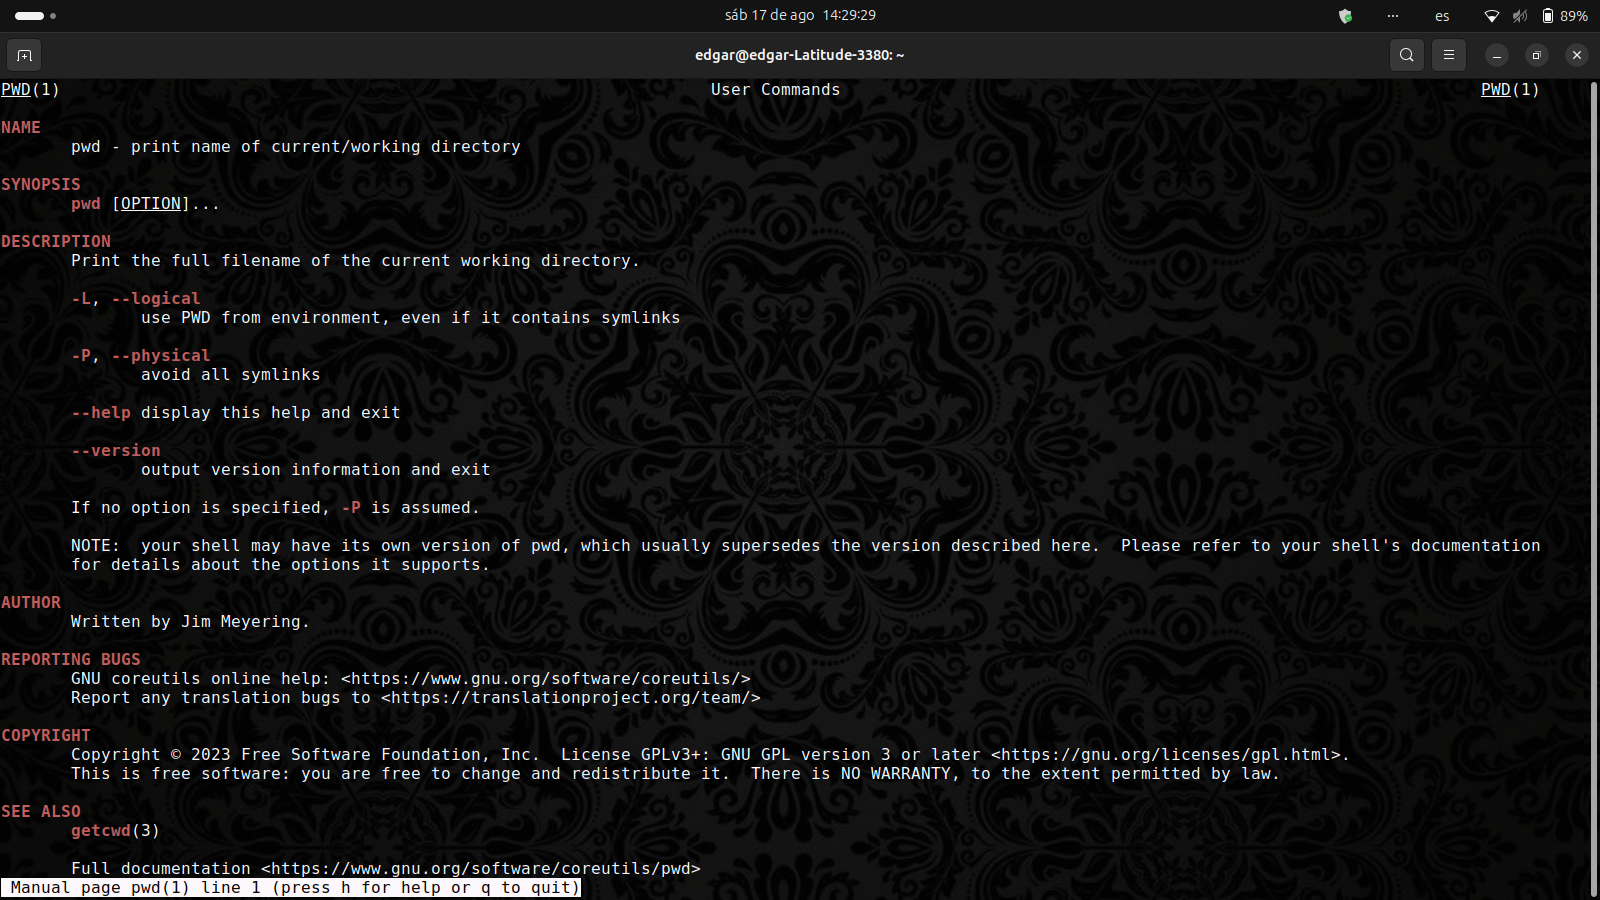
\includegraphics[width=10cm]{IMAGE/man-pwd.png}
    \end{center}
    \begin{itemize}
        \item \texttt{man man}: Muestra el manual del comando \texttt{man}, explicando cómo usar el sistema de páginas de manual.
        \item \texttt{man ls}: Muestra el manual del comando \texttt{ls}, detallando sus opciones y uso.
        \item \texttt{man pwd}: Muestra el manual del comando \texttt{pwd}, que describe cómo obtener el directorio de trabajo actual.
    \end{itemize}

    \item \textbf{mkdir} con 3 banderas \\
    El comando mkdir se utiliza para crear directorios. Y las banderas modifican su comportamiento.\\
    \begin{itemize}
        \item mkdir -v: Muestra un mensaje por cada directorio creado.\\	
        \item mkdir -p: Crea directorios padres si no existen.\\
        \item mkdir -m: Permite asignar permisos al directorio creado.\\
        \item mkdir --help: Muestra la ayuda del comando.\\
    \end{itemize}
    \begin{center}
            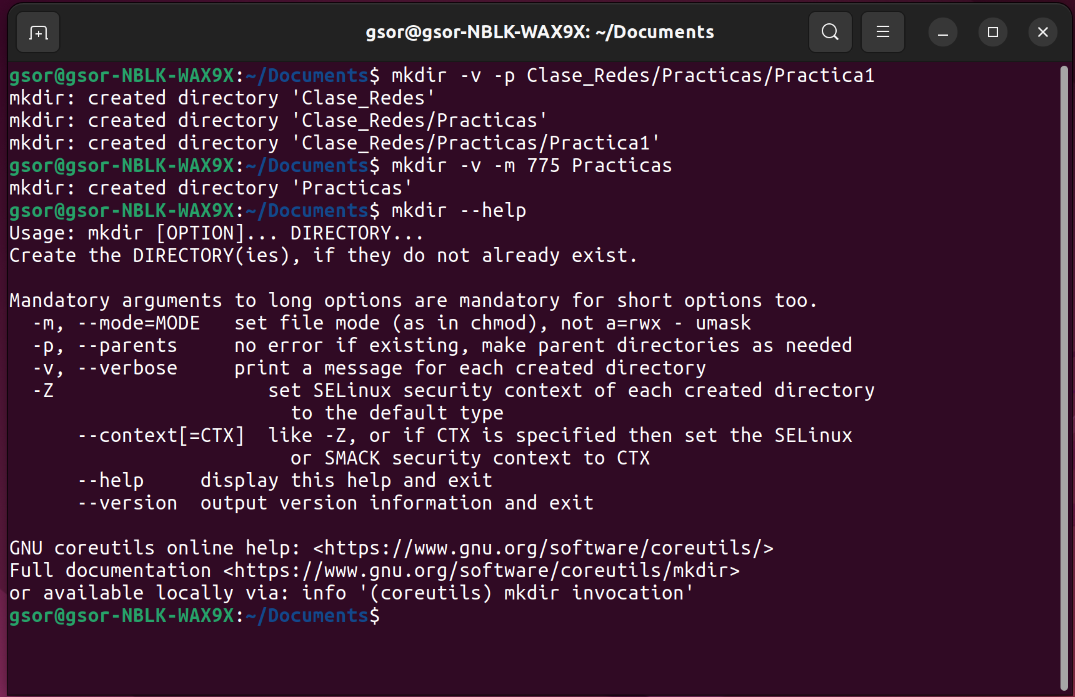
\includegraphics[width=10cm]{IMAGE/comandos/mkdir_examples.png}\\
    \end{center}
    \item \textbf{cp} con al menos 3 banderas
    El comando cp se utiliza para copiar archivos o directorios.\\
    \begin{itemize}
        \item cp -v: Muestra un mensaje por cada archivo copiado.\\
        \item cp -s: Crea un enlace simbólico en lugar de copiar el archivo.\\
        \item cp -t <directorio>: Copia los archivos al directorio especificado.\\
        \item cp -r <directorio>: Copia un directorio y su contenido.\\
    \end{itemize}
    \begin{center}
        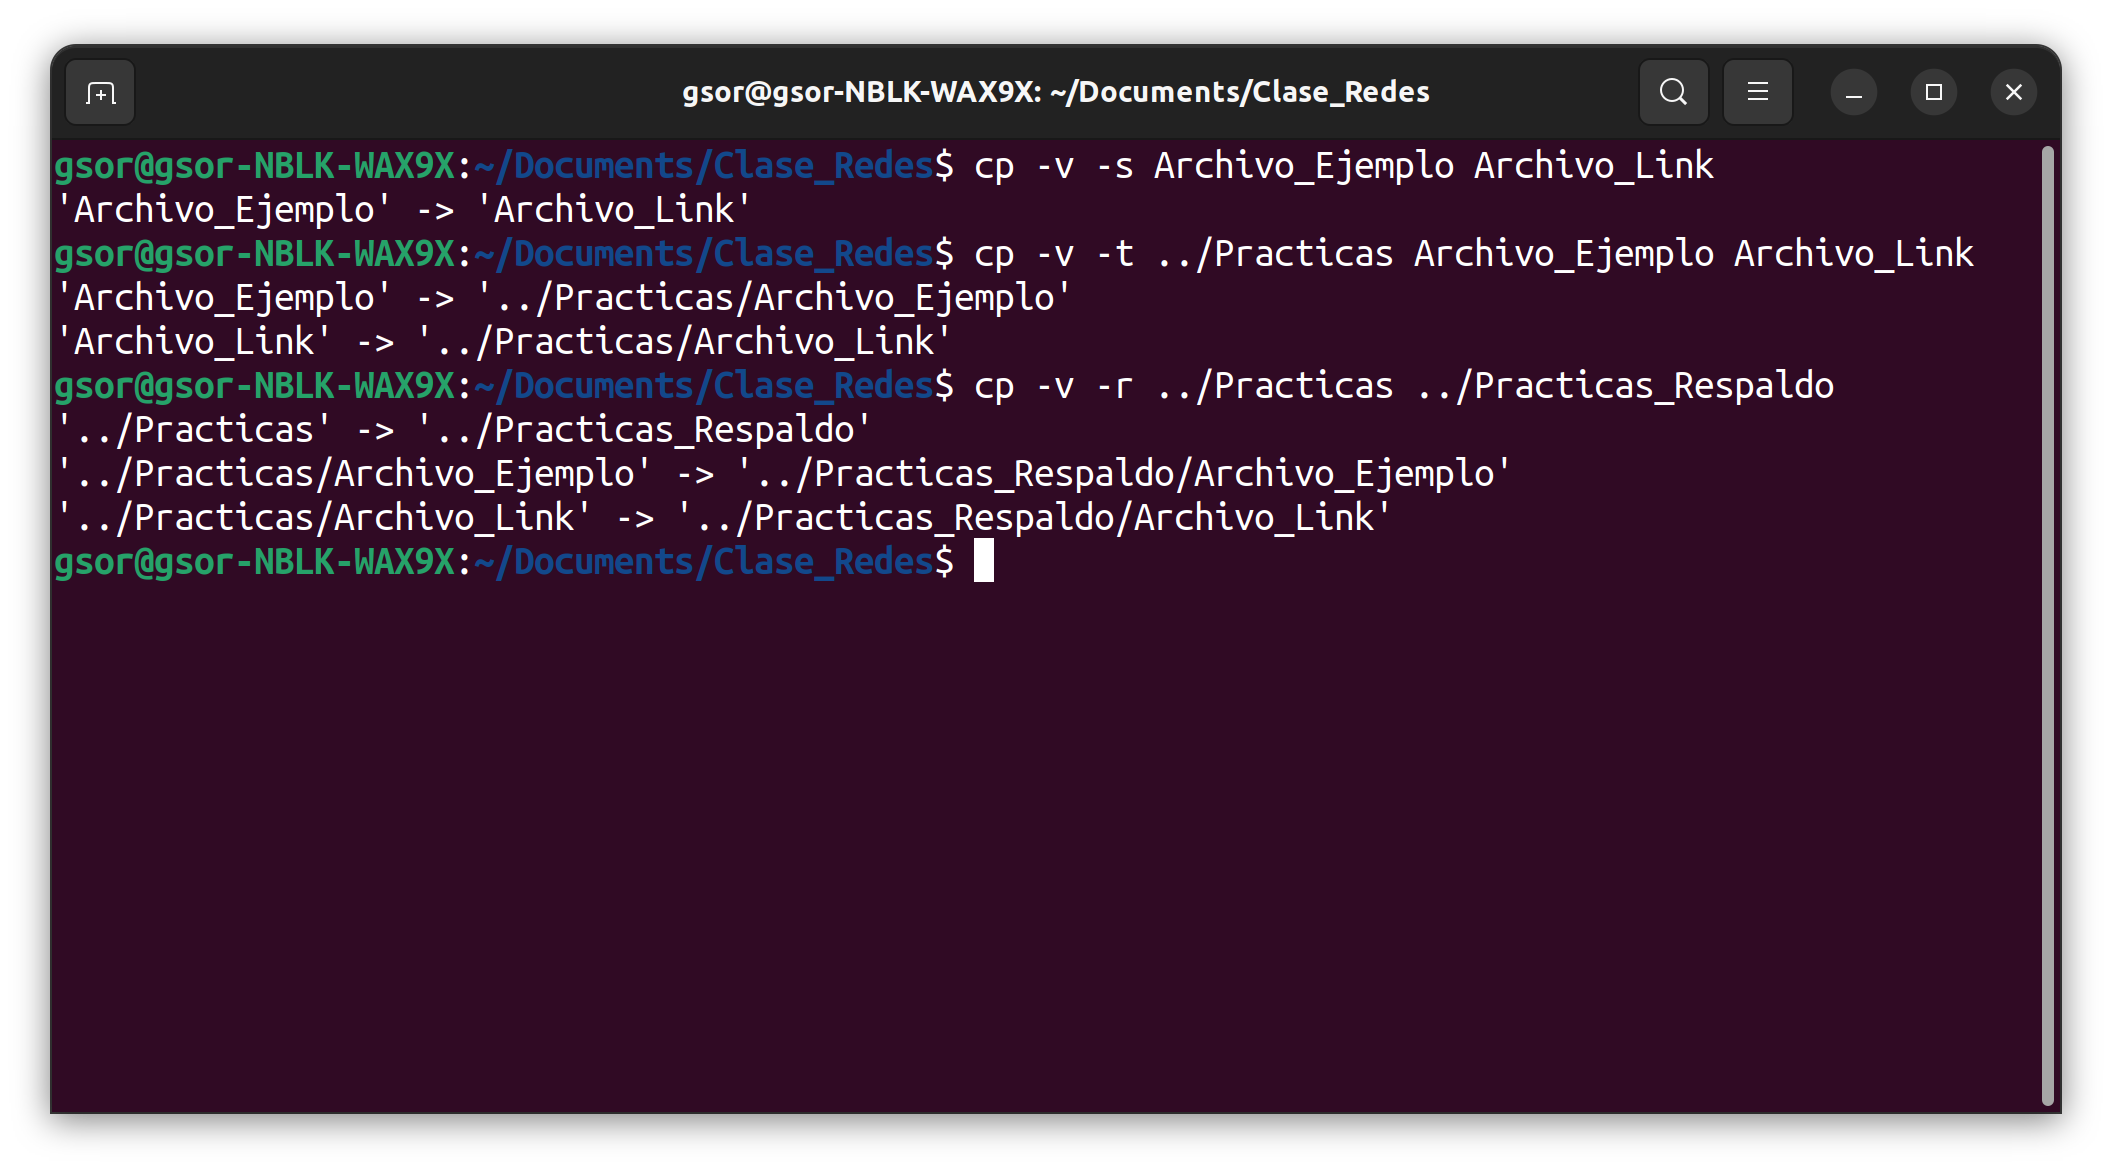
\includegraphics[width=10cm]{IMAGE/comandos/cp_examples.png}\\
    \end{center}
    \item \textbf{mv} con al menos 3 banderas. \\
	Su función principal es mover archivos de un directorio a otro.  También puede renombrar archivos o carpetas. \\
	-v: Explica lo que hace el comando y lo ejecuta.\\
	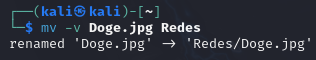
\includegraphics[]{IMAGE/Ejercicio1/mv1.png}\\
	-t: Mueve diferentes archivos a un directorio, primero se escribe el directorio y después los archivos.\\
	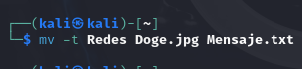
\includegraphics[]{IMAGE/Ejercicio1/mv2.png}\\
	-i: En caso de que el archivo a mover/renombrar ya exista en el directorio destino, pregunta si se quiere sobreescribir.\\
	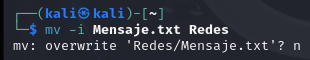
\includegraphics[]{IMAGE/Ejercicio1/mv3.png}\\
    \item \textbf{grep} con al menos 3 banderas. \\
	Su función es buscar un patrón que definamos en un archivo de texto, es decir buscar una o varias palabras en un 
	archivo y se imprimirá la línea o líneas que coincidan.\\
	-i: No distingue minúsculas de mayúsculas.\\
	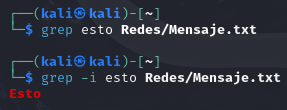
\includegraphics[]{IMAGE/Ejercicio1/grep1.png}\\
	-n: Indica el número de línea donde se encontró el patron.\\
	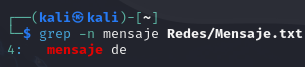
\includegraphics[]{IMAGE/Ejercicio1/grep2.png}\\
	-x: Encuentra el patron donde coincida la linea completa.\\
	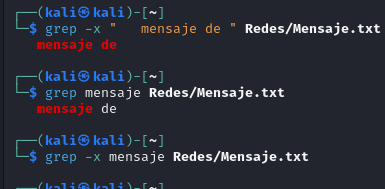
\includegraphics[]{IMAGE/Ejercicio1/grep3.png}\\
    \item \textbf{cat}\\
	Deriva de la palabra concatenar y permite crear, fusionar o imprimir archivos en la terminal.\\
	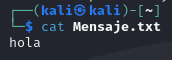
\includegraphics[]{IMAGE/Ejercicio1/cat.png}\\
    \item \textbf{head} (con alguna configuración)\\
	Sirve para mostrar el inicio de un archivo de texto.\\
	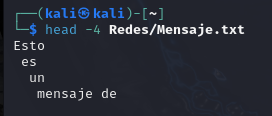
\includegraphics[]{IMAGE/Ejercicio1/head.png}\\
    \item \textbf{less} (con alguna configuración)
    Es un visor de archivos que permite desplazarse por el contenido de un archivo de texto.\\
    \begin{itemize}
        \item less -N:  Muestra los números de línea junto al contenido del archivo.\\
    \end{itemize}
    \begin{center}
        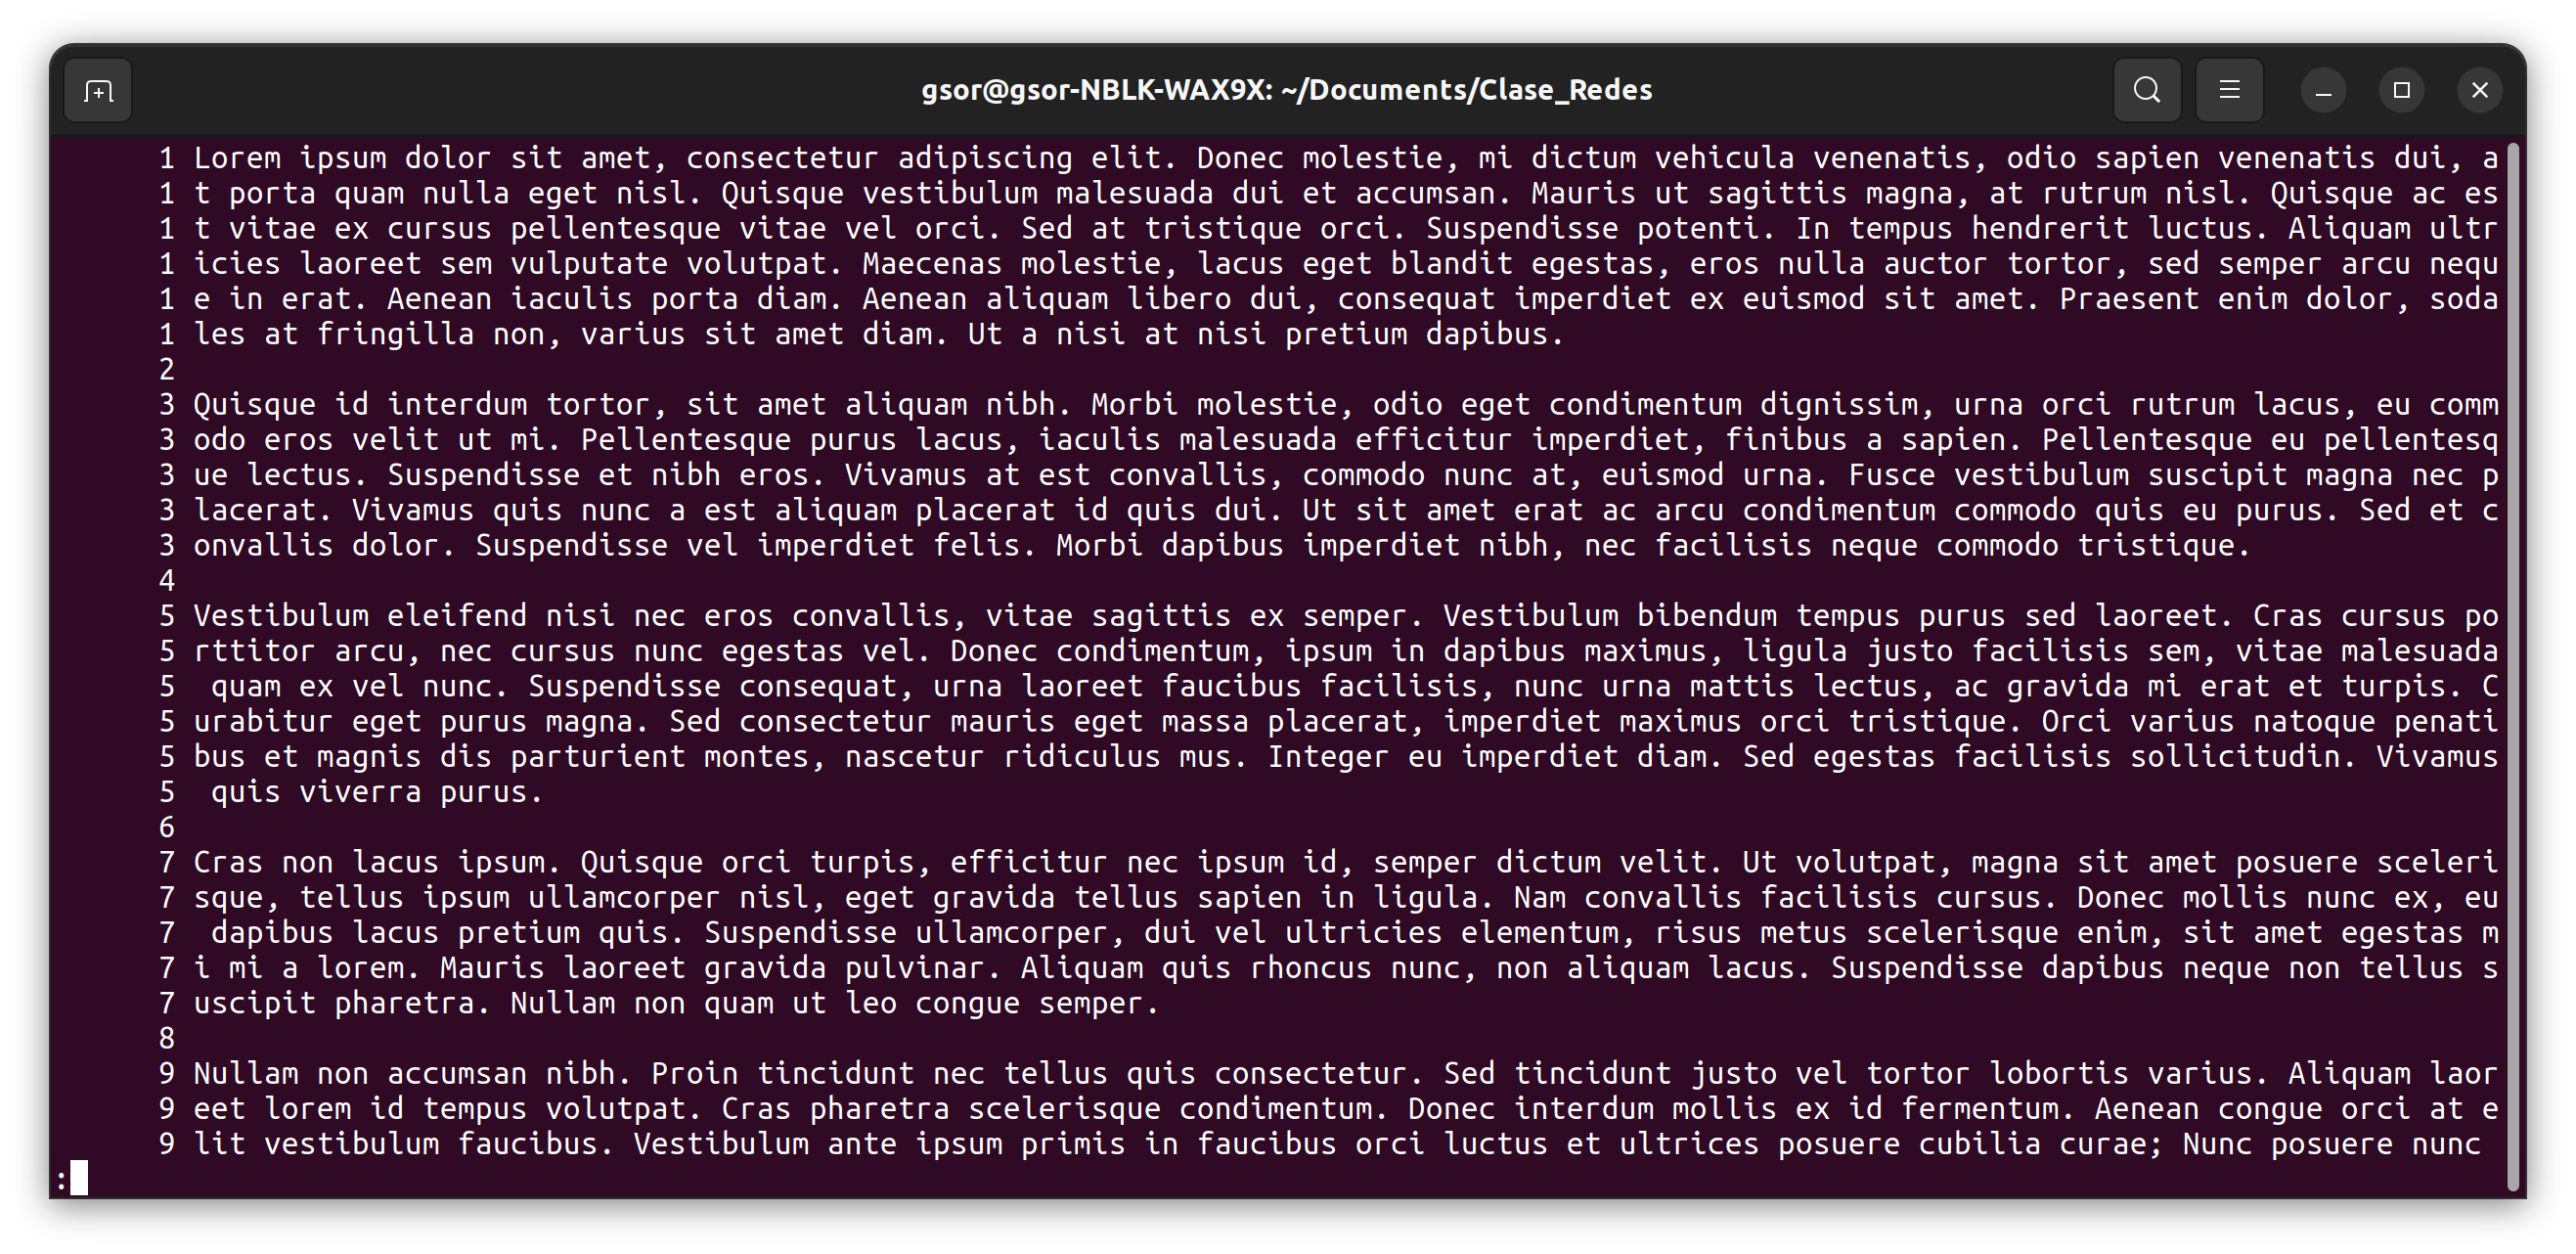
\includegraphics[width=10cm]{IMAGE/comandos/less-example.png}\\
    \end{center}
    \item \textbf{find}\\
    Busca archivos que cumplan las condiciones que especifique el usuario, comenzando por el directorio que nombre. Por ejemplo, si quiere buscar nombres de archivos que concuerden con determinado patrón o que hayan sido modificados durante un periodo de tiempo determinado.\\
    \begin{center}
        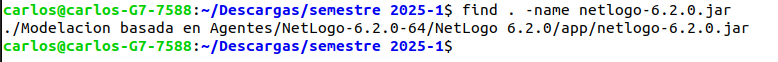
\includegraphics[width=12cm]{IMAGE/find.png}
    \end{center}
    
    \item \textbf{uniq}\\
    Permite obtener líneas únicas de un archivo o entrada dada. Elimina líneas consecutivas duplicadas, dejando solo una de ellas.
    \begin{center}
        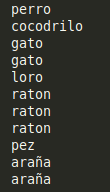
\includegraphics[width=2cm]{IMAGE/lista.png}
    \end{center}
    
    \begin{center}
        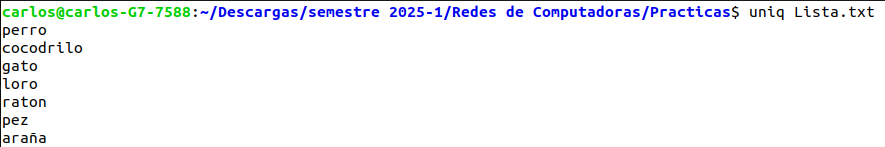
\includegraphics[width=13cm]{IMAGE/uniq.png}
    \end{center}
    
    \item \textbf{ps}; ¿Qué significará PID y TTY?\\
    Muestra una lista con todos los procesos que se estén ejecutando en el sistema en ese momento, con su identificador del proceso (PID), terminal asociado (TTY), tiempo de uso de CPU (TIME) y nombre del ejecutable (CMD).
    \begin{center}
        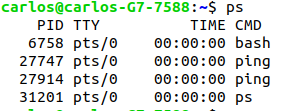
\includegraphics[width=5cm]{IMAGE/ps.png}
    \end{center}
    \item \textbf{kill}, ¿Tendrá relación con \textbf{ps}?
    El comando kill se utiliza para enviar una señal a un proceso, por lo general para detenerlo.\\
    \begin{itemize}
        \item less -N:  Muestra los números de línea junto al contenido del archivo.\\
    \end{itemize}
    \begin{center}
         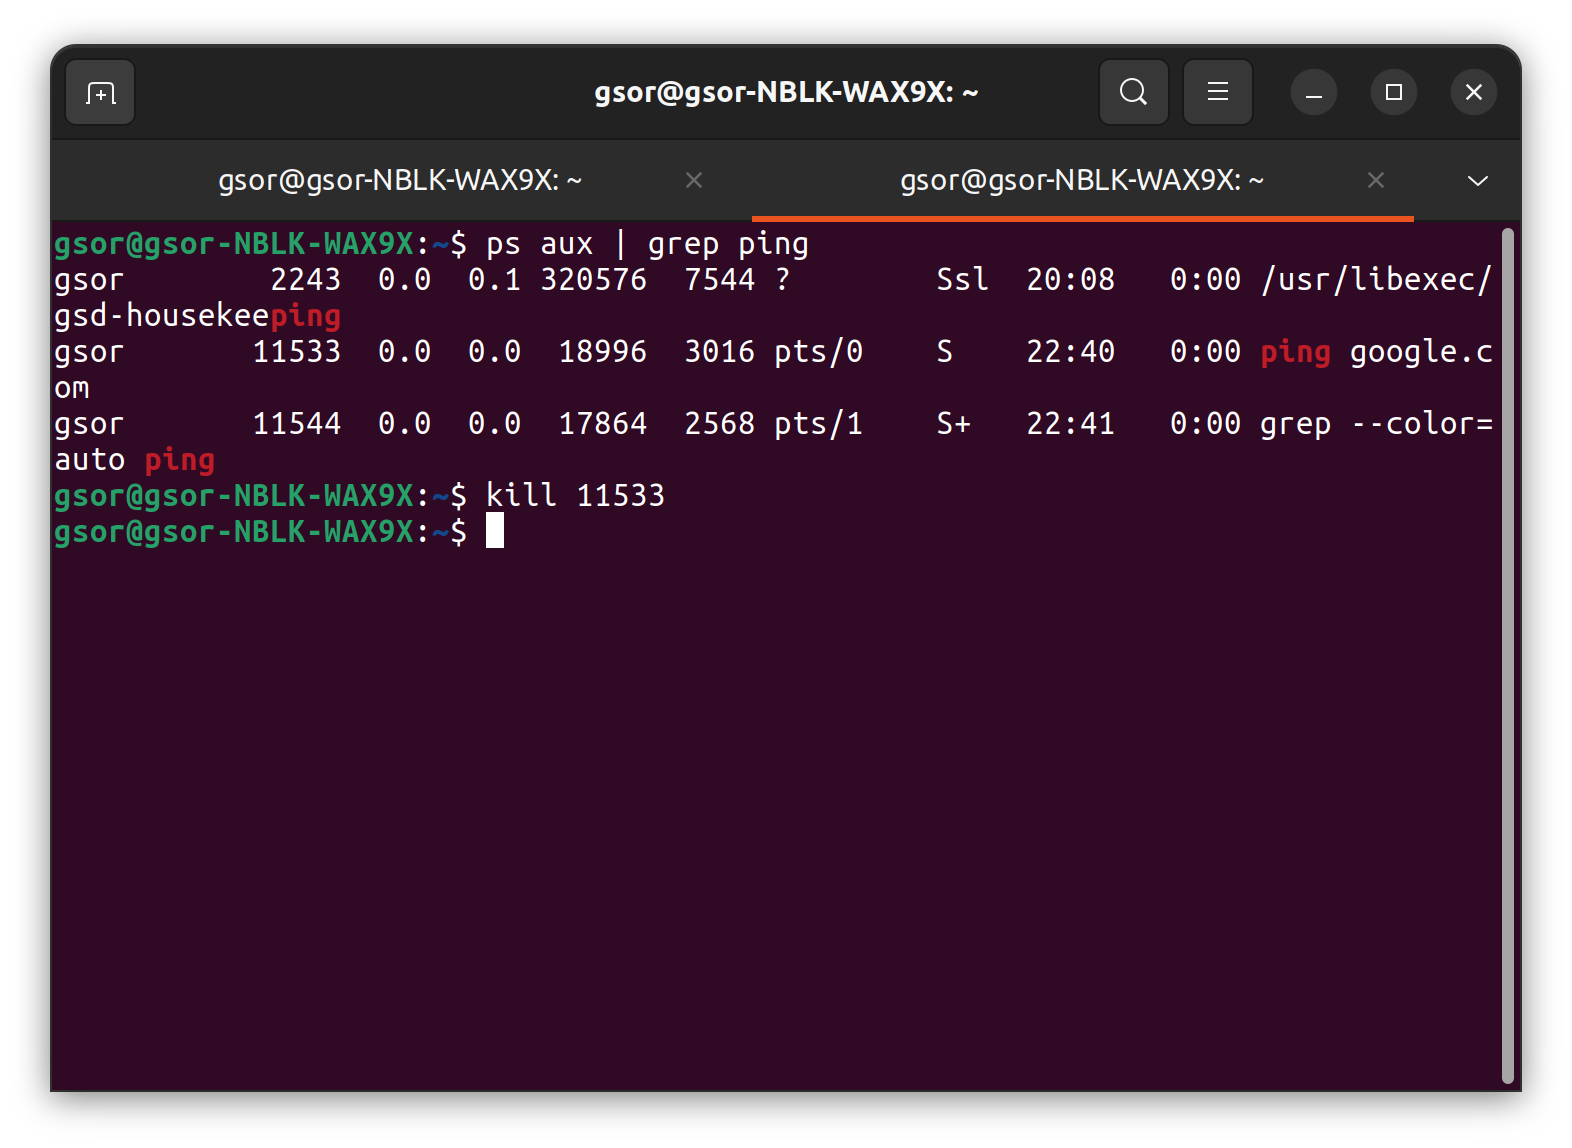
\includegraphics[width=10cm]{IMAGE/comandos/kill.png}\\
    \end{center}
    Para poder usar el comando kill es necesario conocer el PID del proceso que se desea detener, para ello se usa el comando ps.\\
    \item \textbf{1}
    El comando df se utiliza para mostrar el espacio disponible en los sistemas de archivos.\\
    \begin{itemize}
        \item df -h: Muestra el espacio disponible en los sistemas de archivos en un formato legible para el usuario.\\
        \item df -T: Muestra el tipo de sistema de archivos.\\
        \item df -i: Muestra el número de inodos disponibles. Un inodo es una estructura de datos utilizada por los sistemas de archivos 
        en Unix y Linux para almacenar información sobre un archivo o un directorio. \\
    \end{itemize}
    \begin{center}
        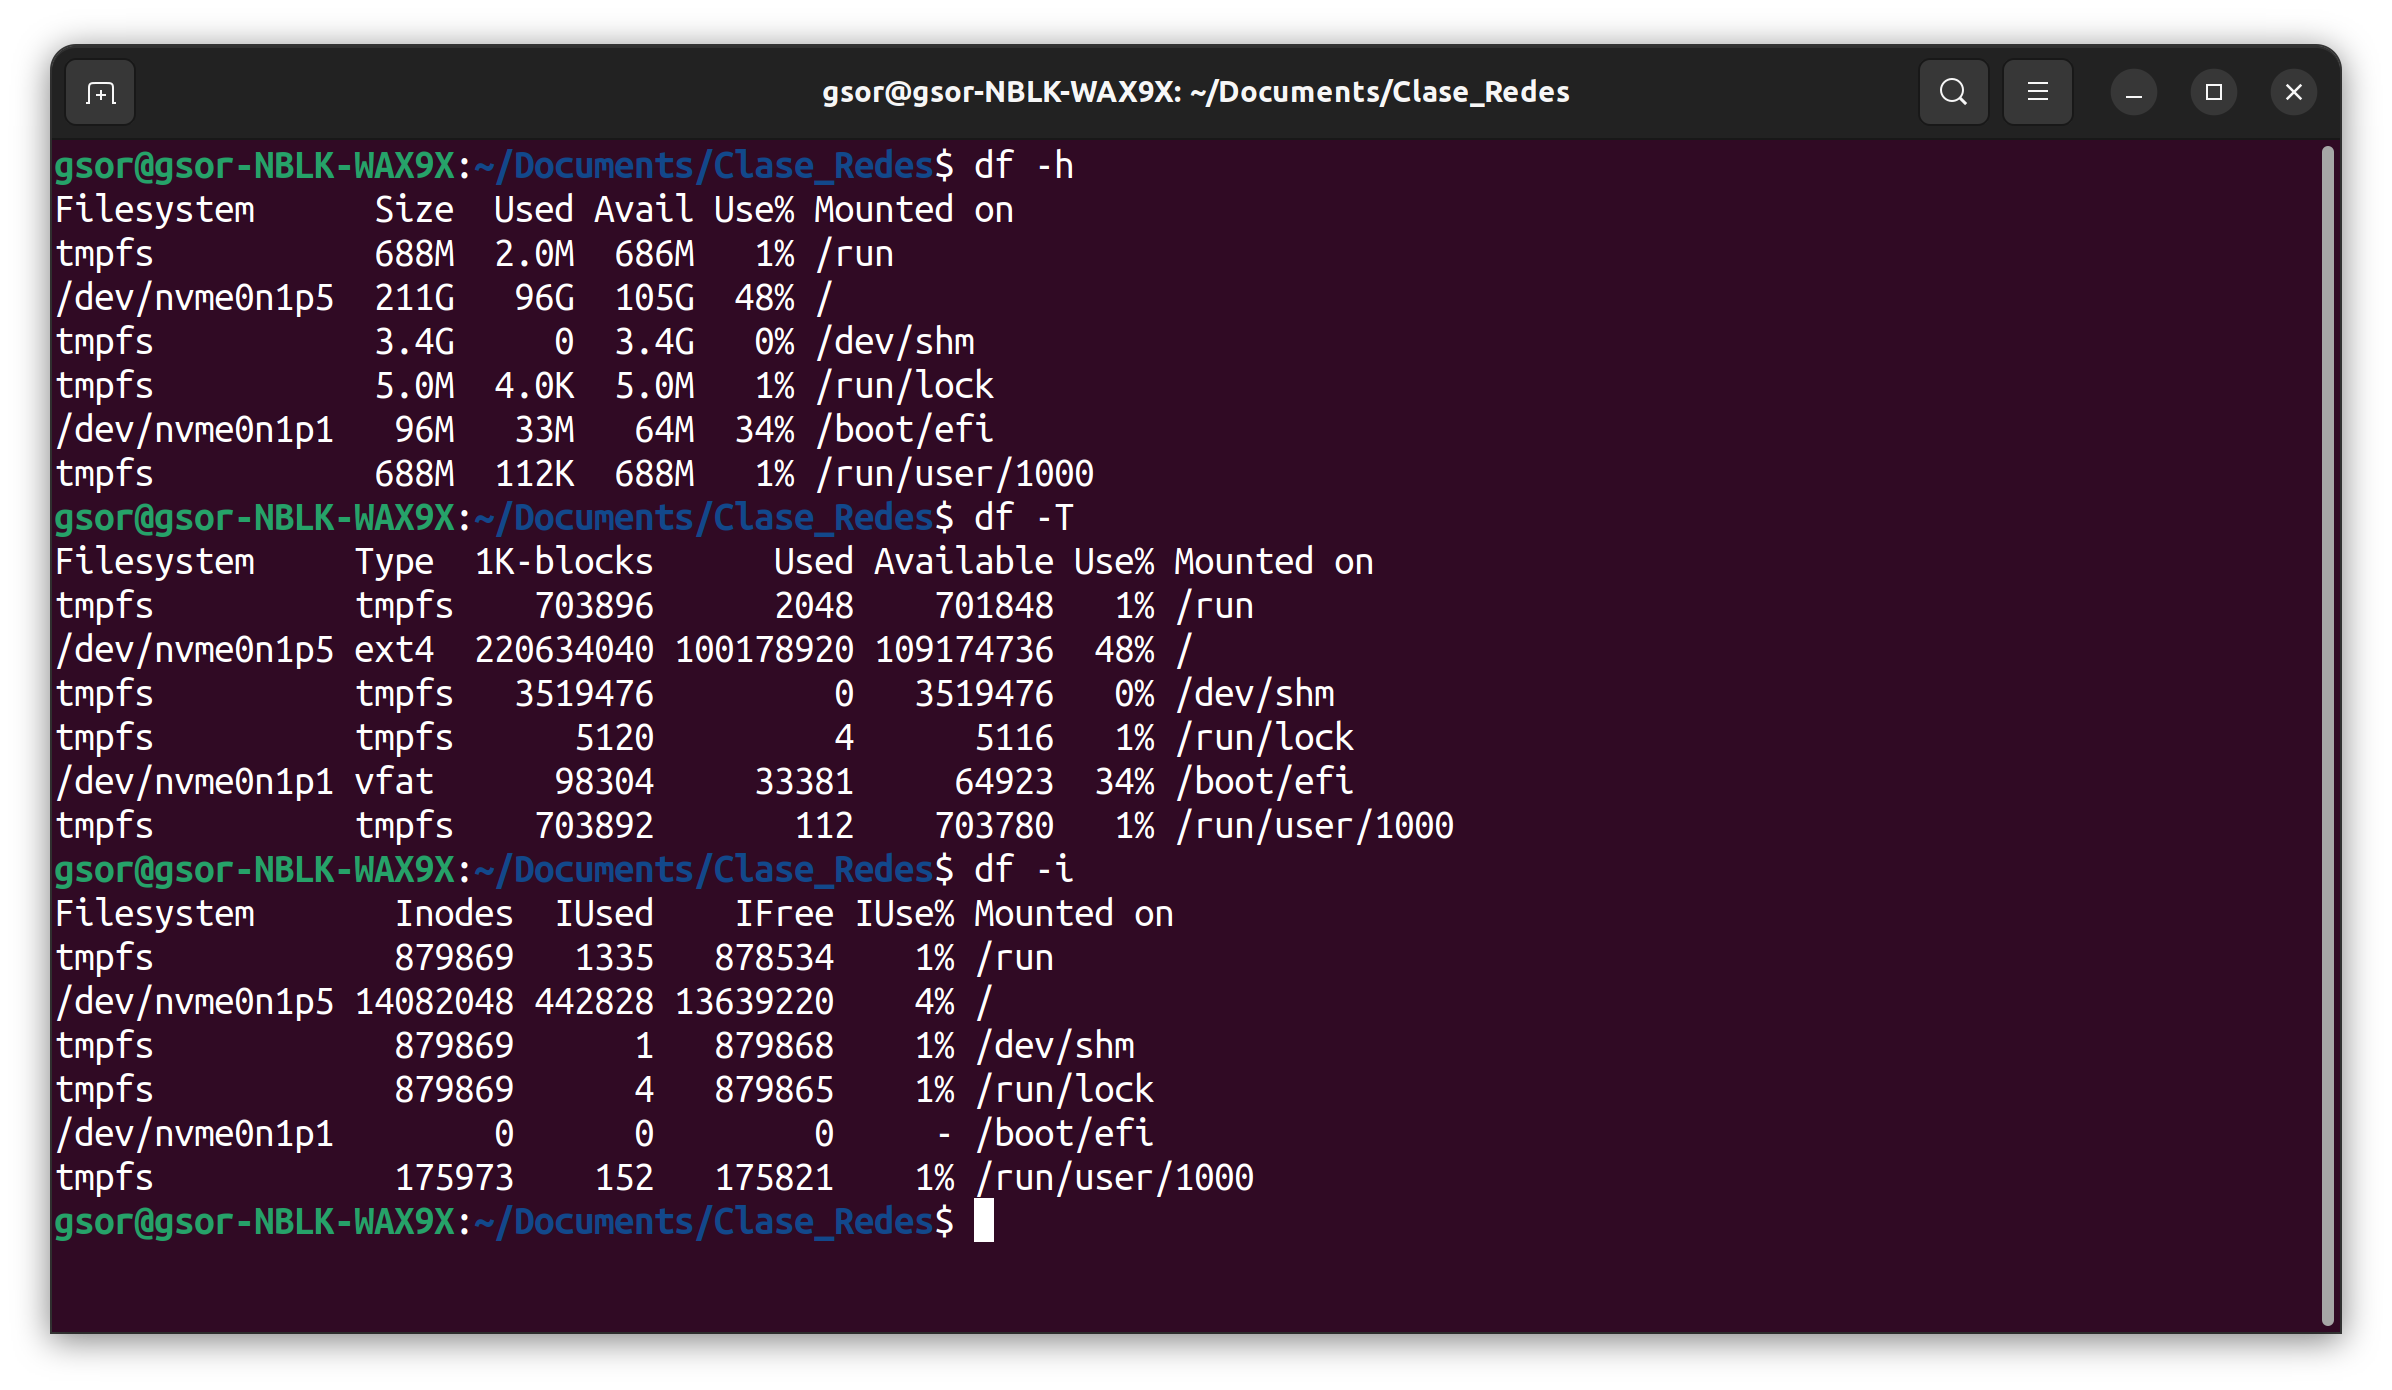
\includegraphics[width=10cm]{IMAGE/comandos/df.png}\\
    \end{center}
    \item \textbf{2}
    El comando curl se utiliza para transferir datos desde o hacia un servidor.\\
    \begin{itemize}
        \item curl -I: Muestra solo la cabecera de la respuesta del servidor.\\
        \item curl -o: Guarda la salida en un archivo en un archivo de texto.\\
        \item curl -L: Sigue redirecciones.\\ 
    \end{itemize}
    \begin{center}
        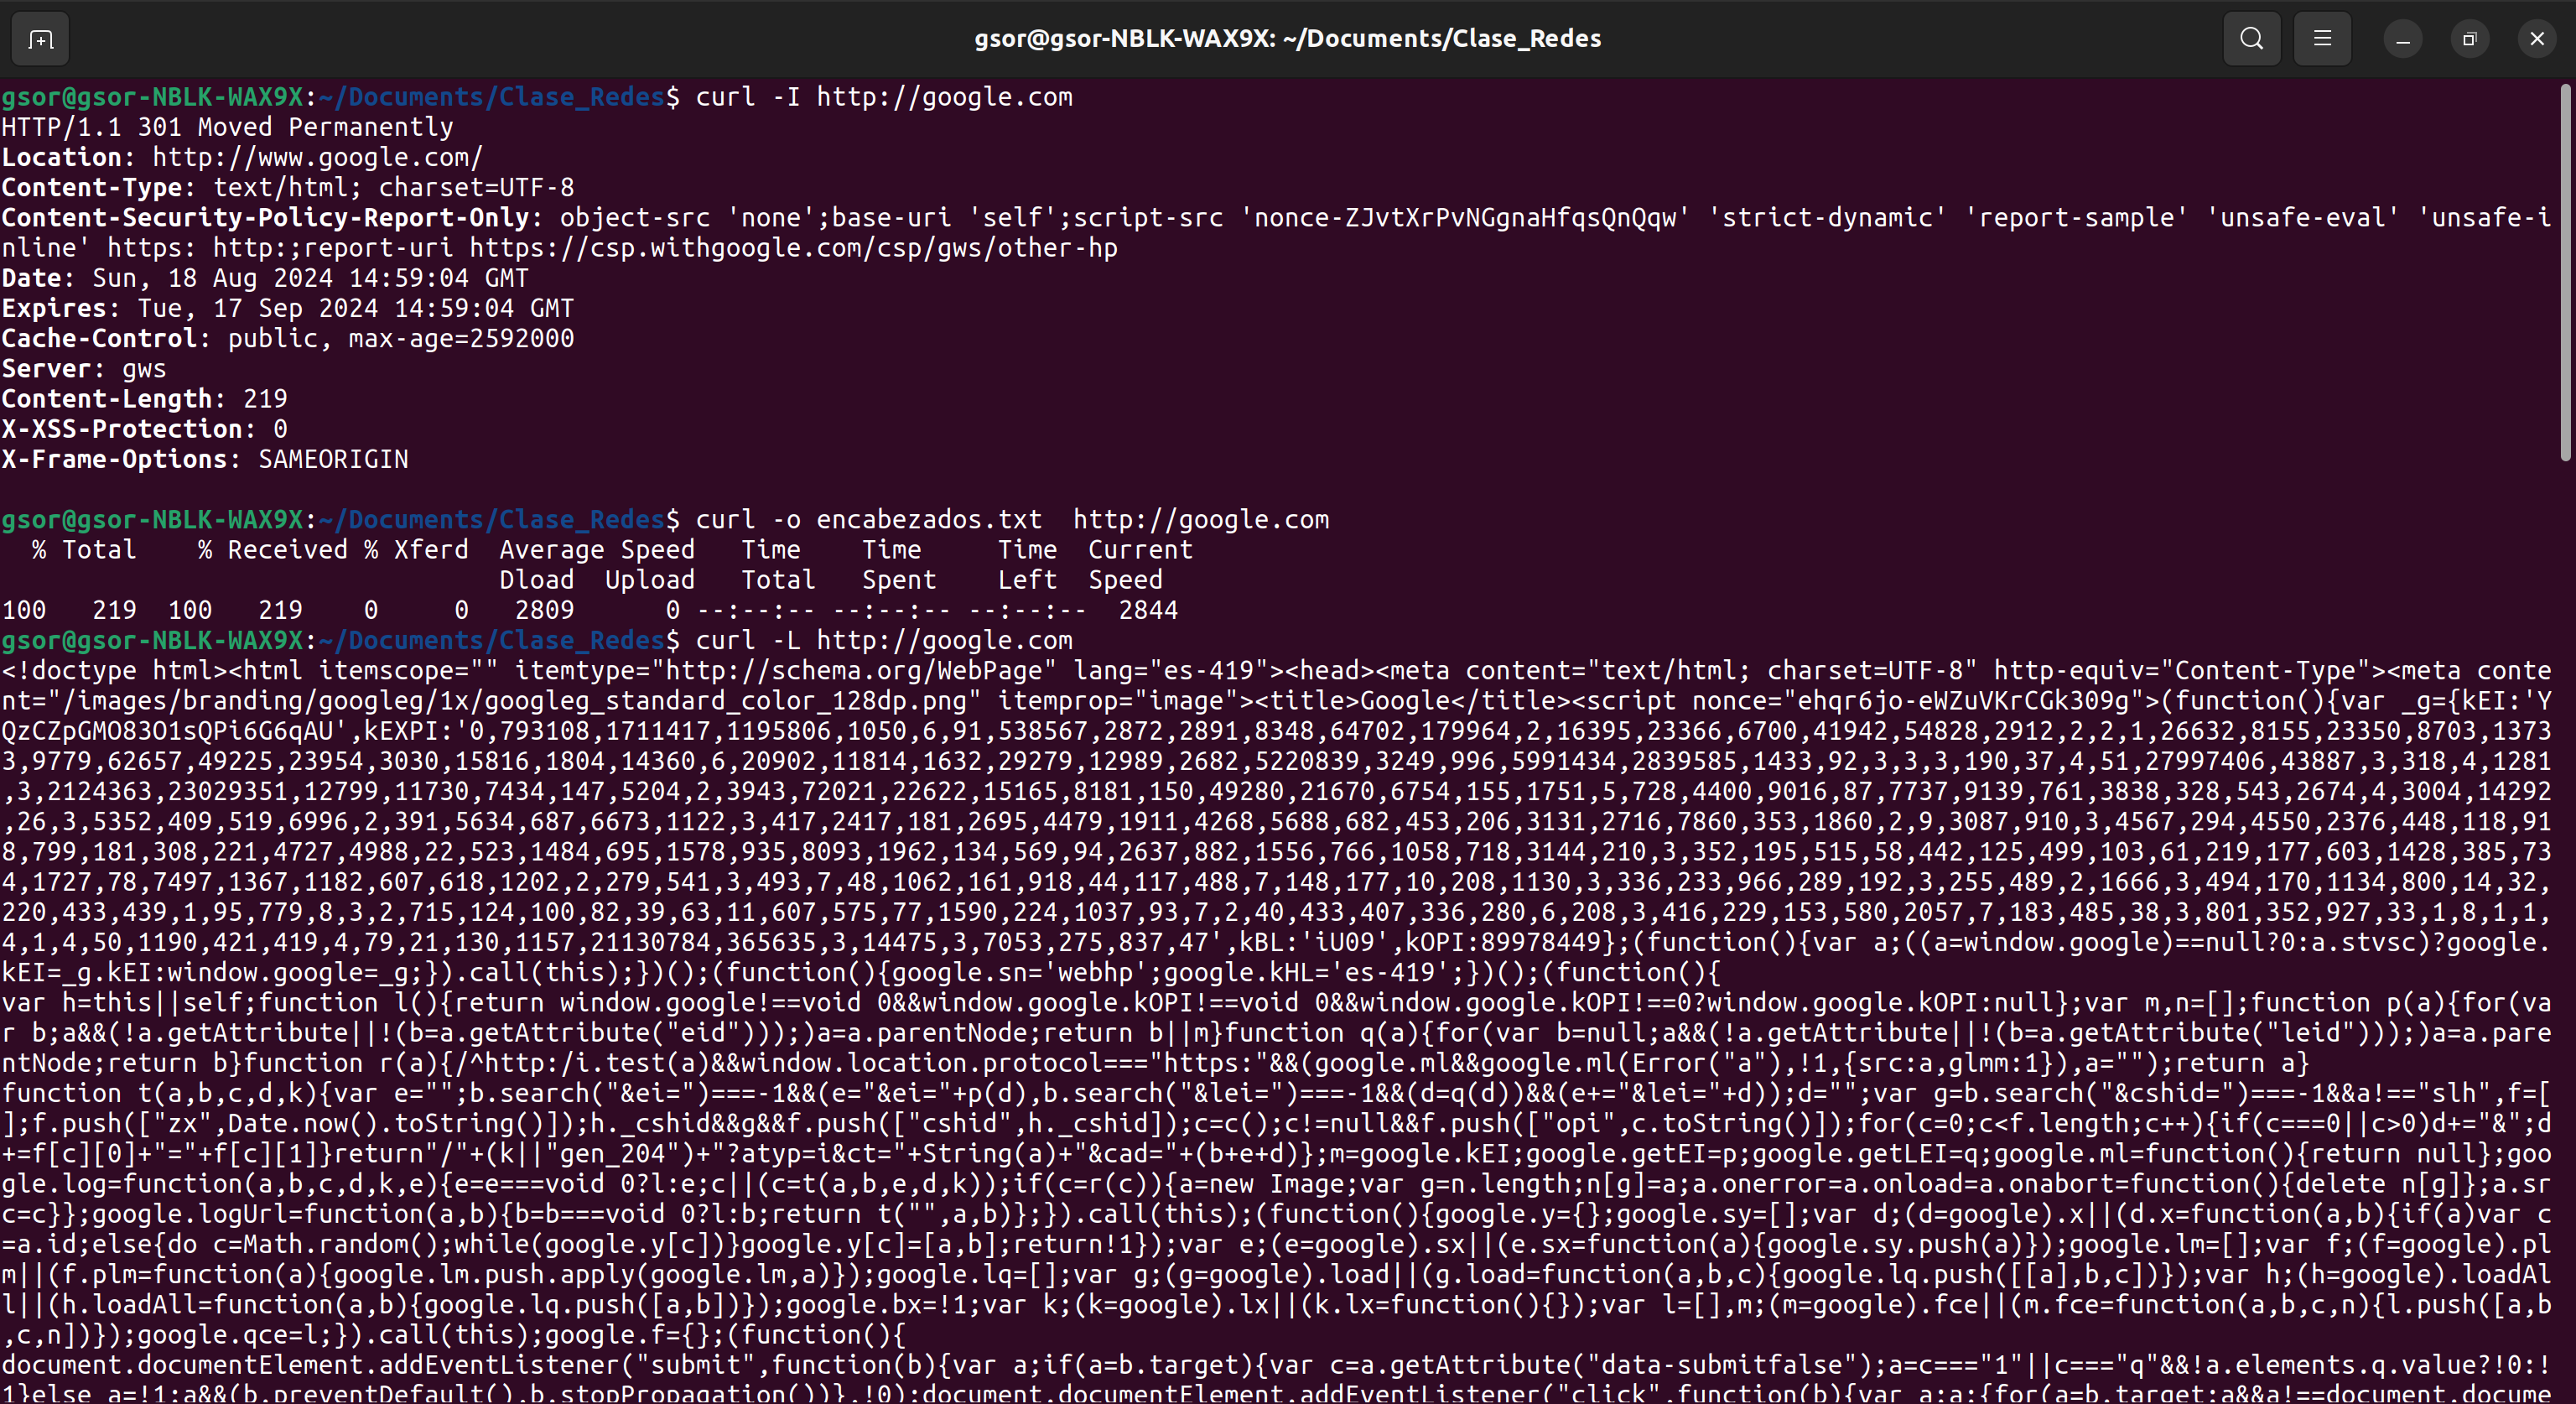
\includegraphics[width=10cm]{IMAGE/comandos/curl.png}\\
    \end{center}
    \item \textbf{3}
    El comando sort se utiliza para ordenar líneas de texto en un archivo.\\
    \begin{itemize}
        \item sort -r: Ordena las líneas en orden inverso.\\
        \item sort -n: Ordena las líneas numéricamente.\\
        \item sort -k <número>: Ordena las líneas por la columna especificada.\\         
    \end{itemize}
    \begin{center}
        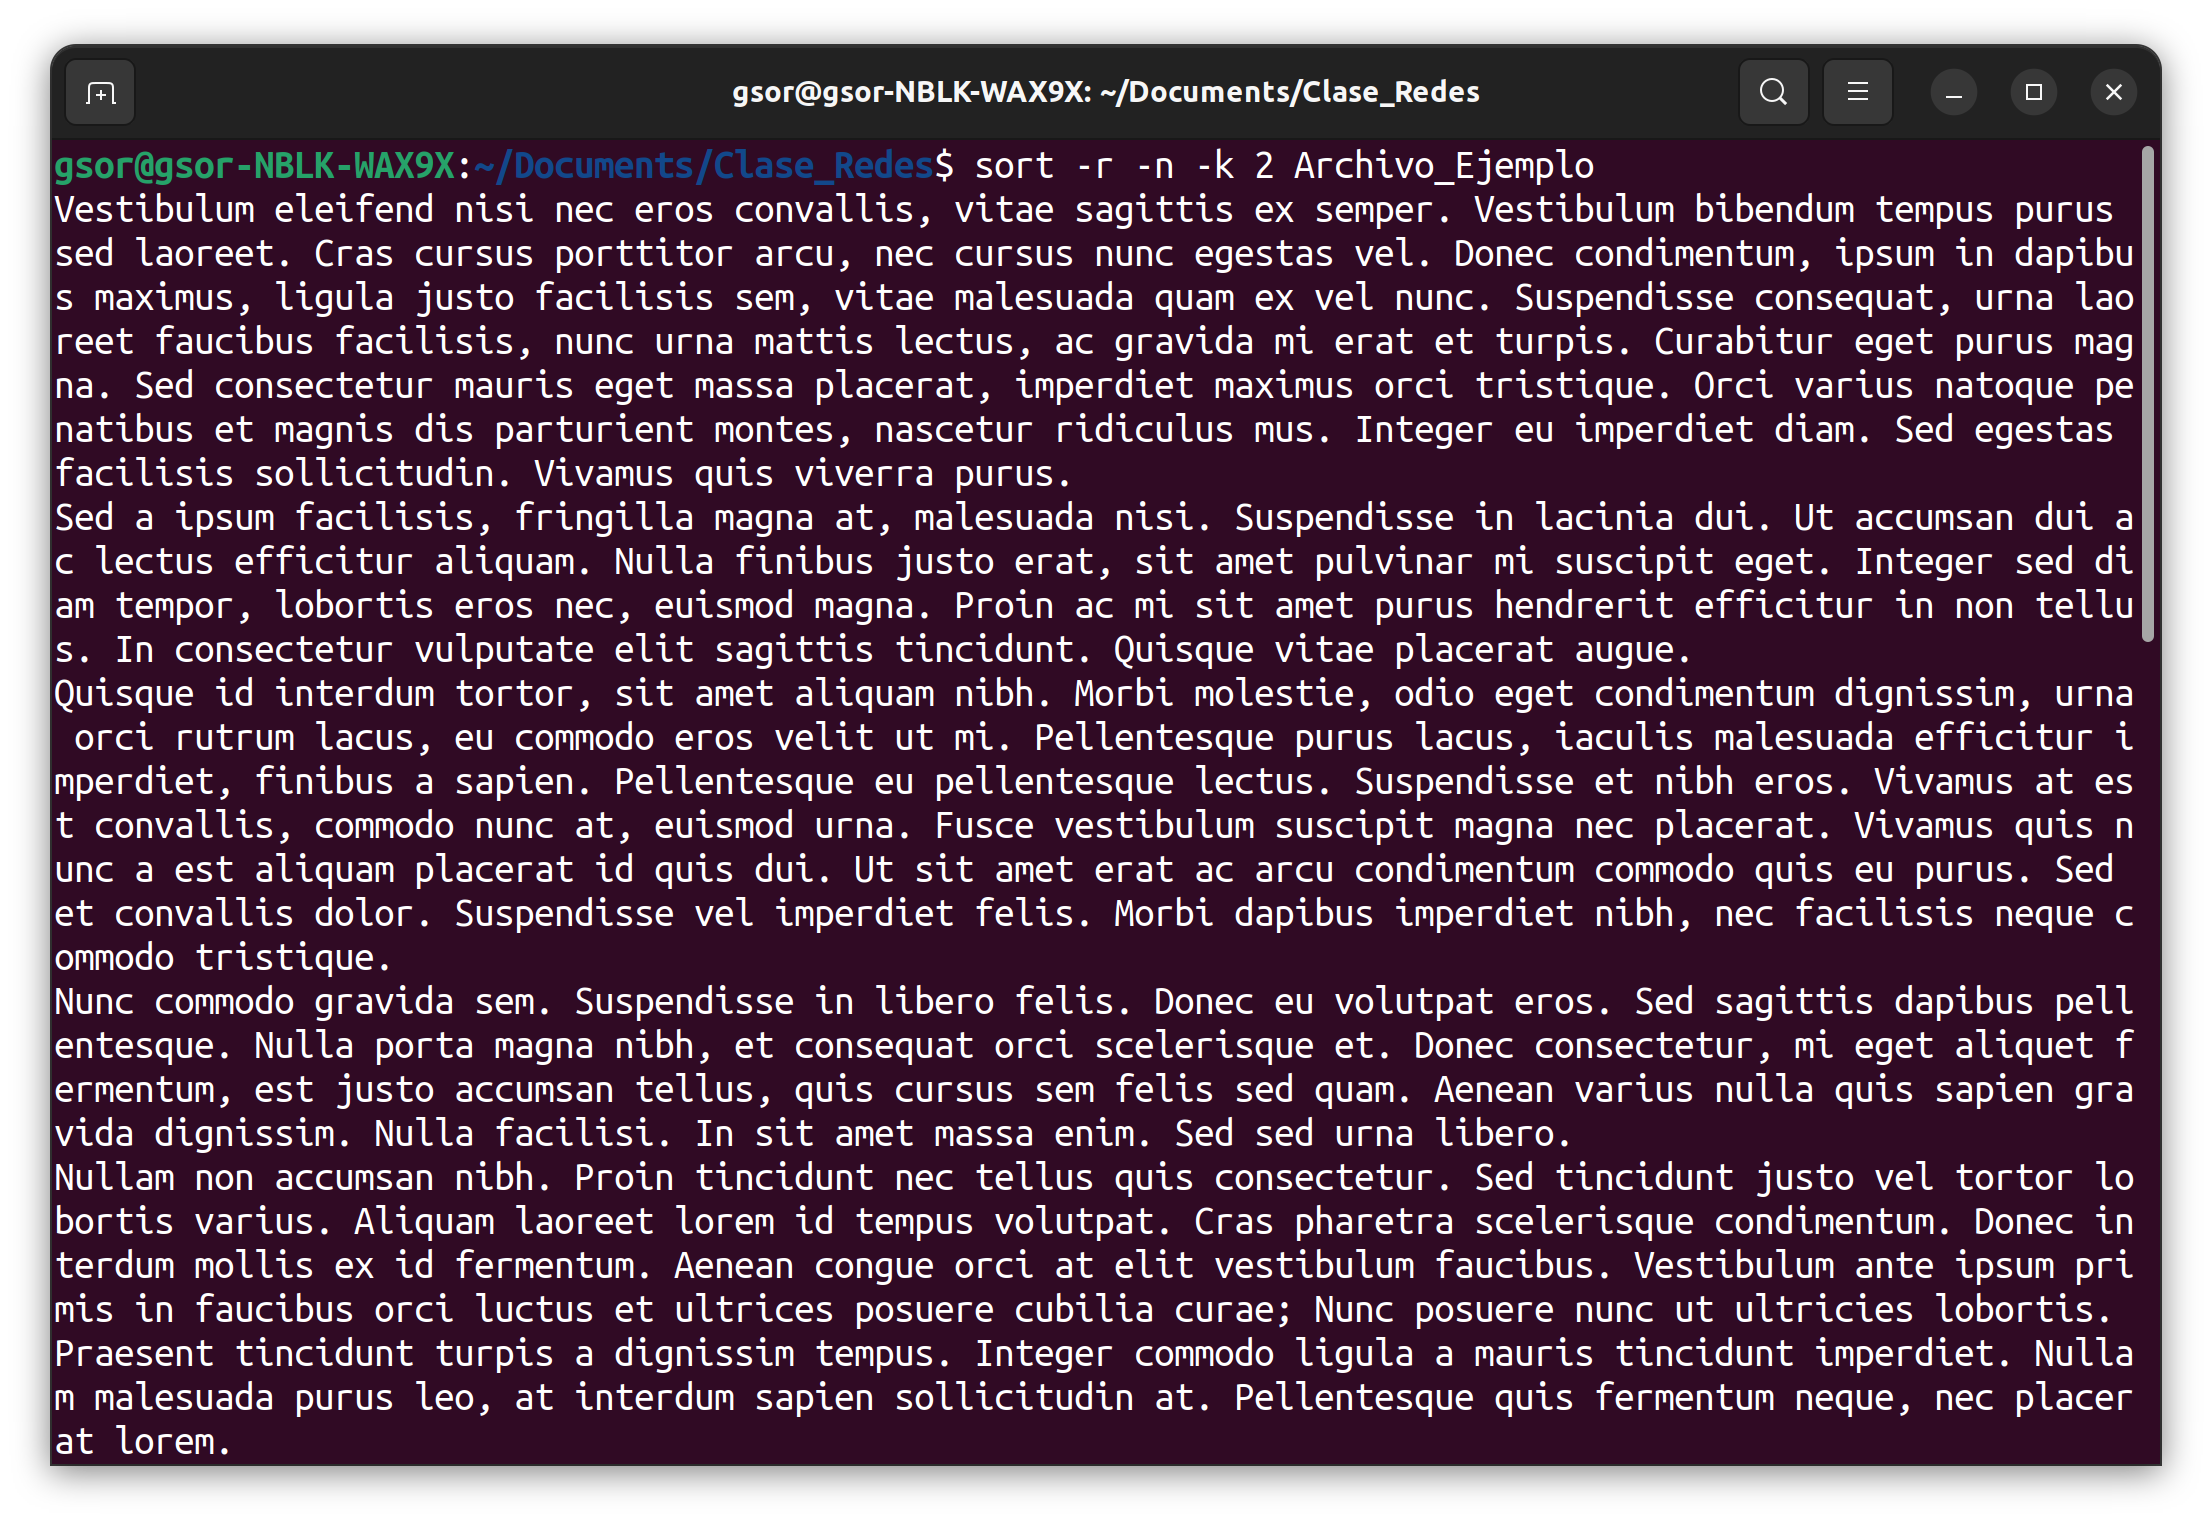
\includegraphics[width=10cm]{IMAGE/comandos/sort.png}\\
    \end{center}
    \item \textbf{4}
    El comando tar se utiliza para comprimir y descomprimir archivos.\\
    \begin{itemize}
        \item tar -c: Crea un archivo comprimido.\\
        \item tar -v : Muestra los archivos que se están comprimiendo o descomprimiendo.\\
        \item tar -f <archivo>: Especifica el nombre del archivo comprimido.\\
        \item tar -z: Comprime o descomprime el archivo con gzip.\\
        \item tar -x: Descomprime un archivo.\\
    \end{itemize}
    \begin{center}
        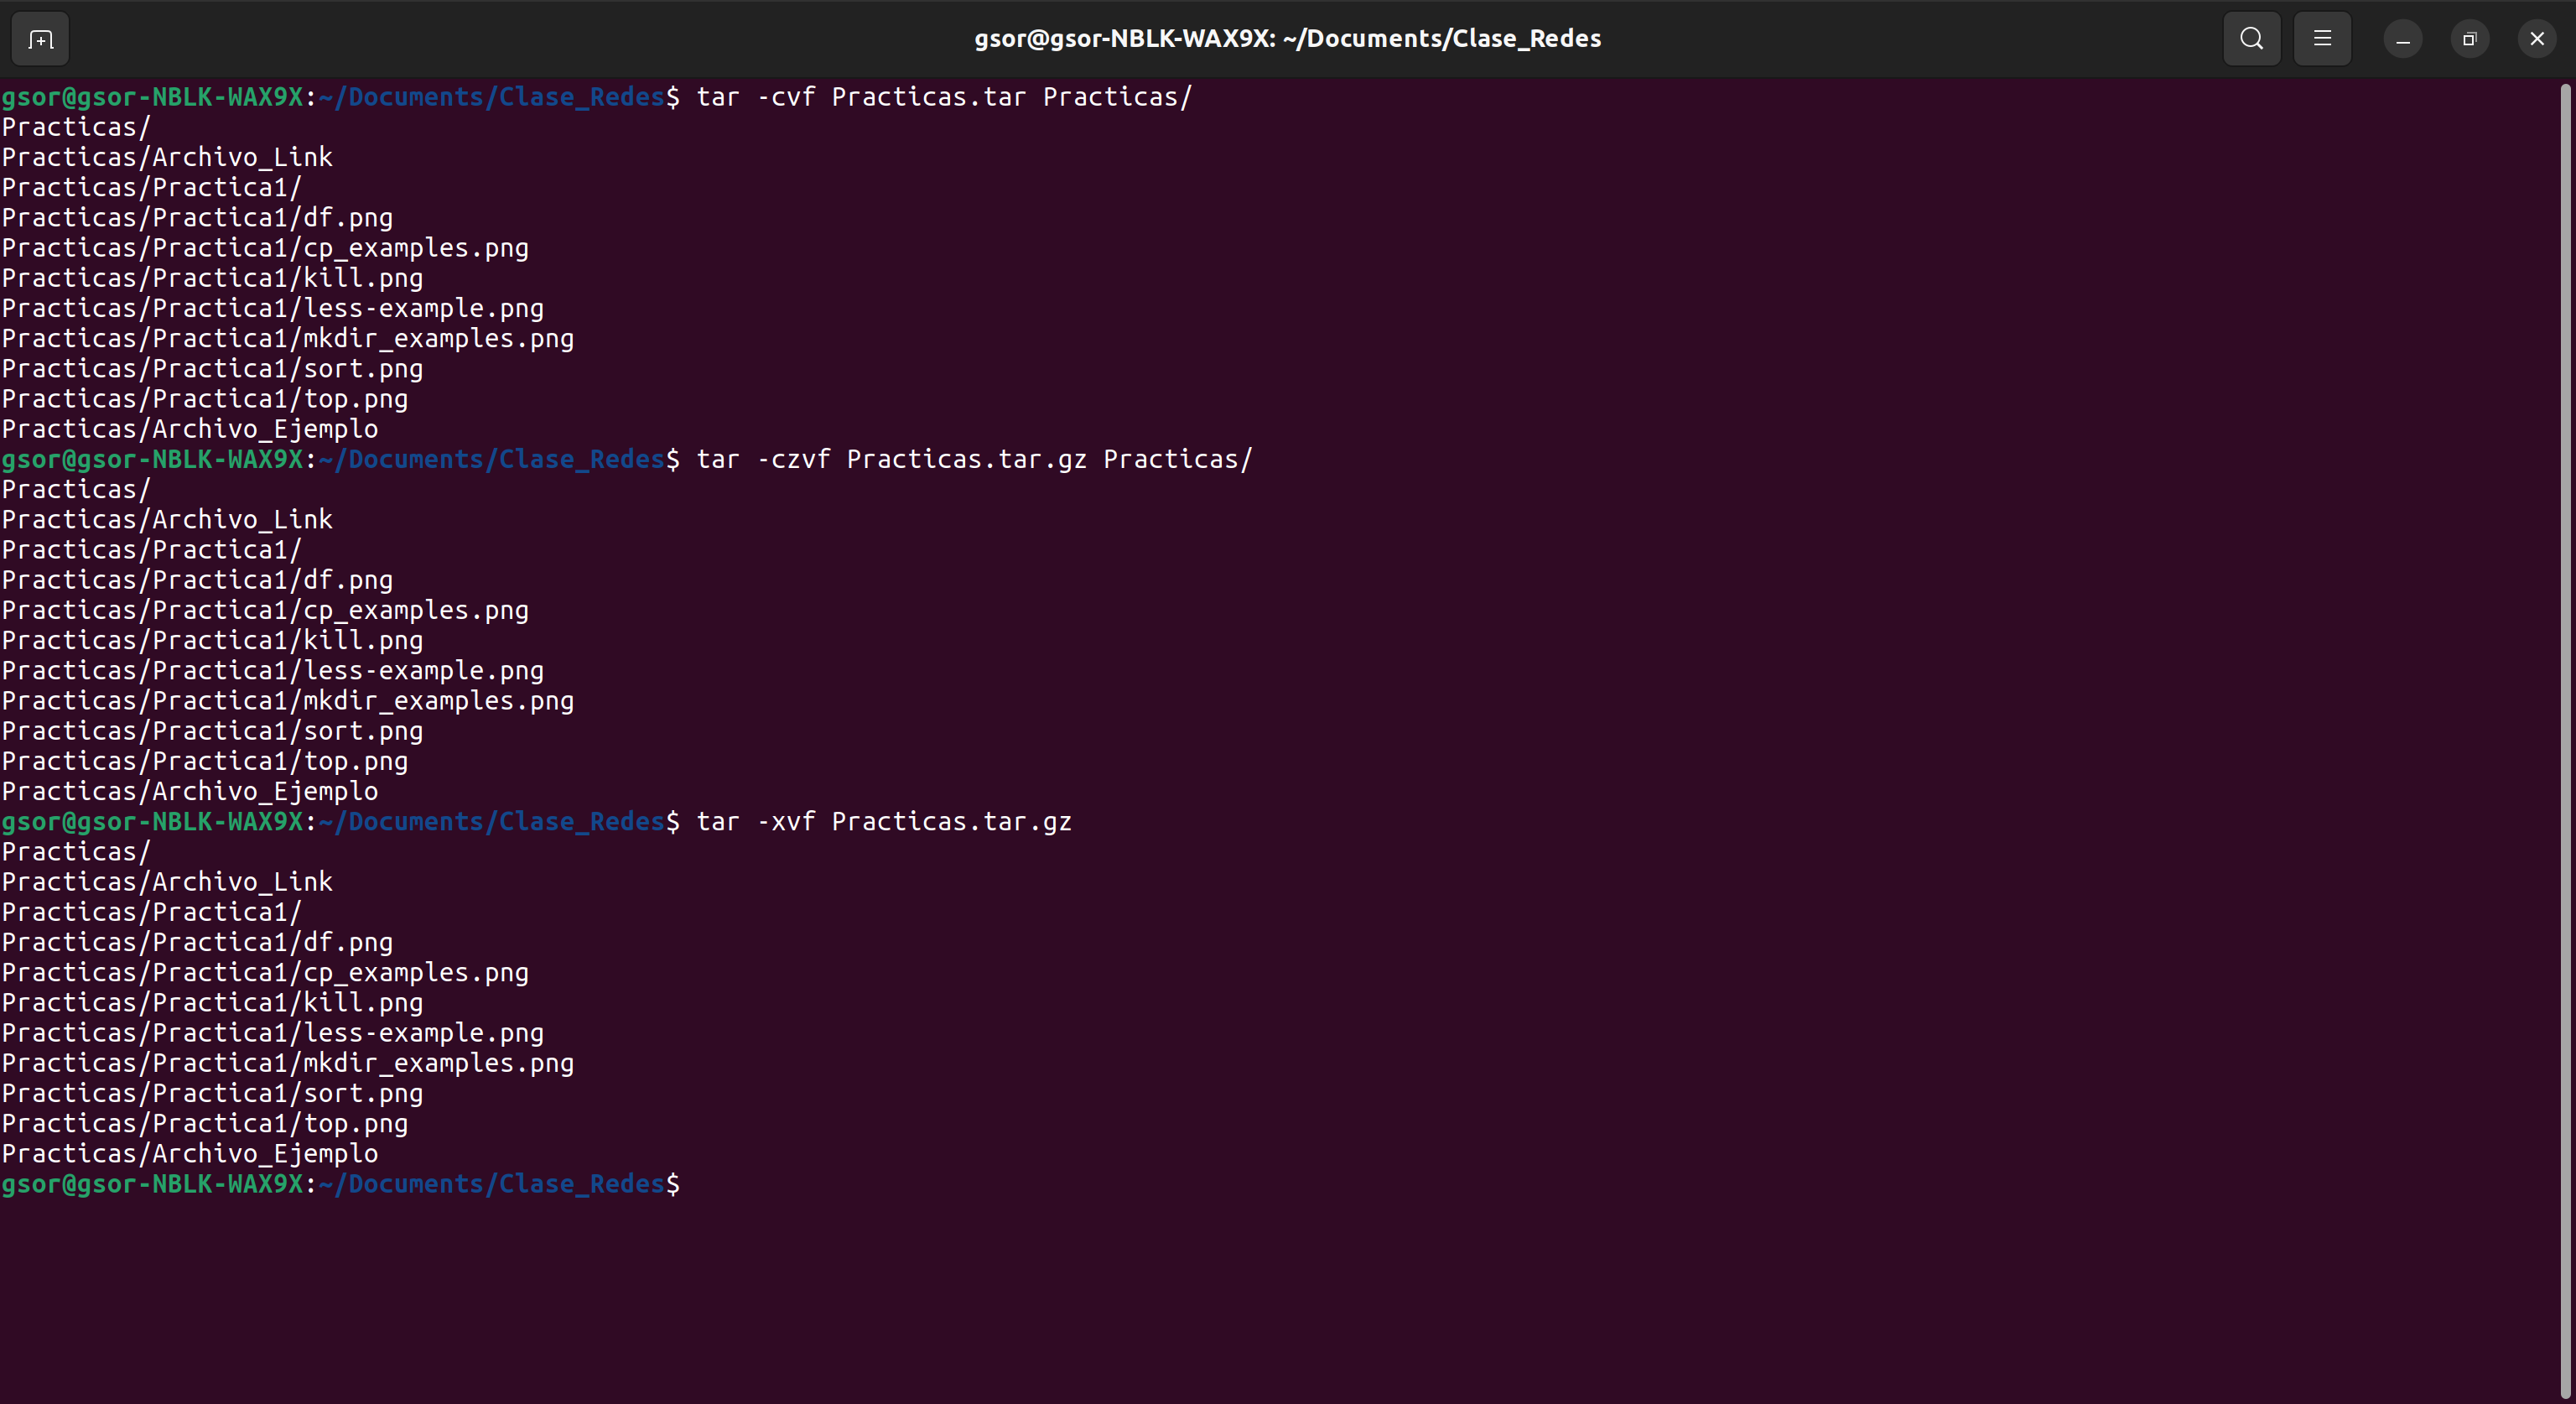
\includegraphics[width=10cm]{IMAGE/comandos/tar.png}\\
    \end{center}
    \item \textbf{5}
    El comando top se utiliza para mostrar los procesos en ejecución en el sistema.\\
    \begin{itemize}
        \item top -d <número>: Actualiza la información cada n segundos.\\
        \item top -u <usuario>: Muestra los procesos del usuario especificado.\\
        \item top -b : Muestra la información en modo batch.\\
    \end{itemize}
    \begin{center}
        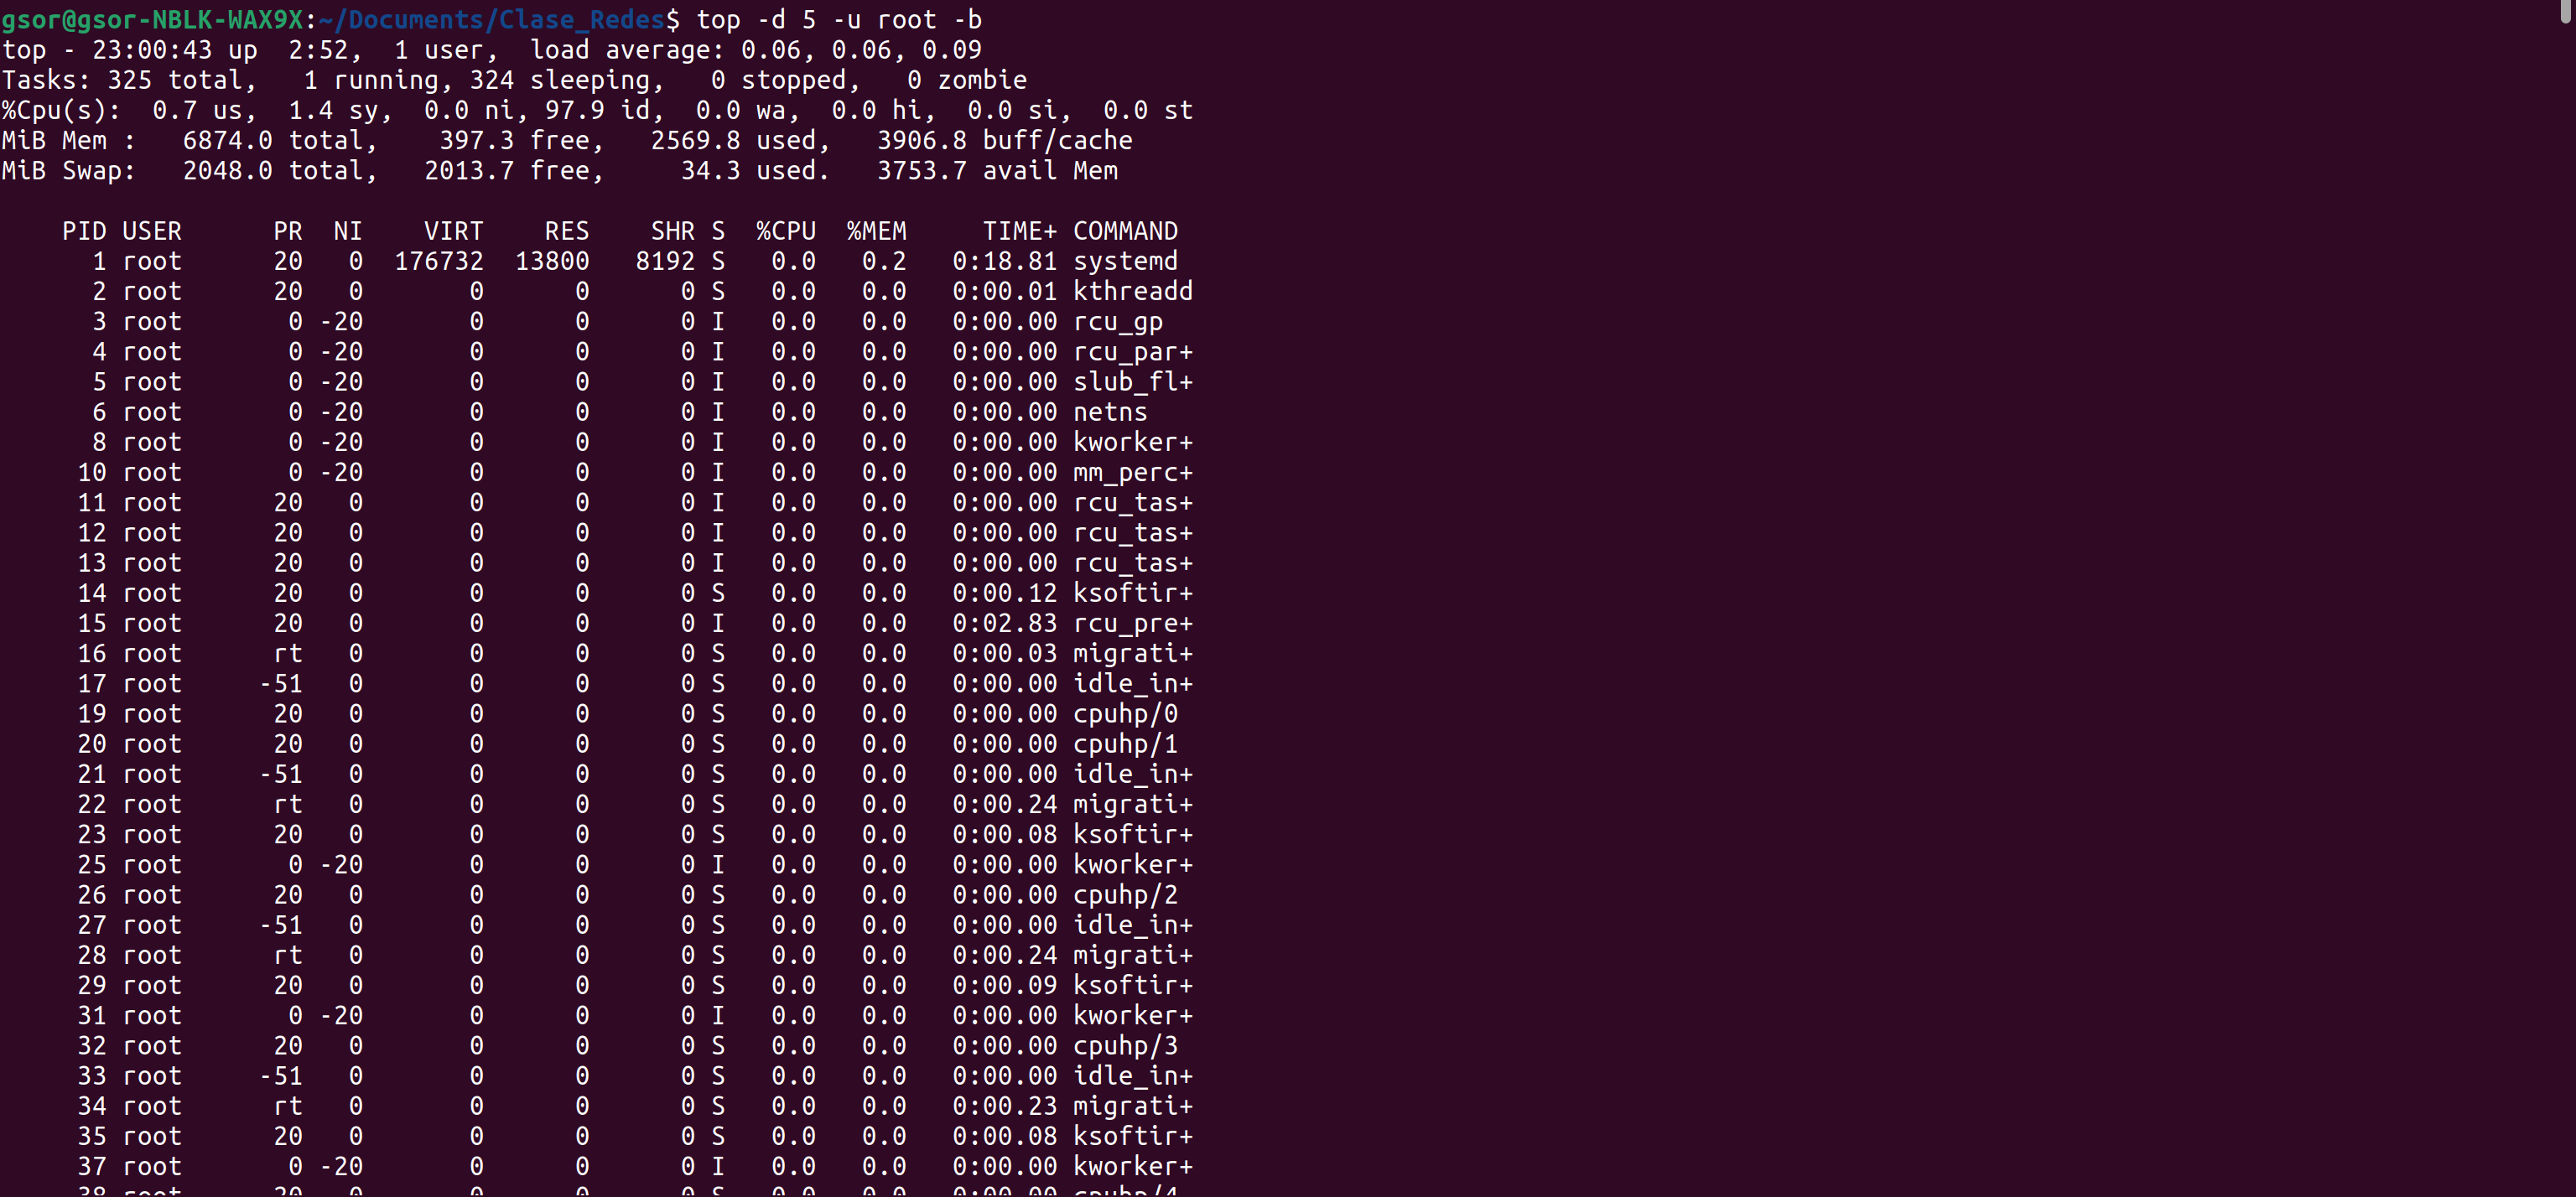
\includegraphics[width=10cm]{IMAGE/comandos/top.png}\\
    \end{center}
\end{itemize}